% !TEX program = xelatex
\documentclass[usenames,dvipsnames, 10pt]{beamer}
\usefonttheme{serif}
\usefonttheme{structuresmallcapsserif}
\usetheme{Warsaw}
\usepackage{xcolor}
\beamertemplatenavigationsymbolsempty
\usepackage{tikz}
\usepackage{pgfplots}
\renewcommand{\qed}{\hfill\blacksquare}
\newcommand{\D}[1]{\Delta #1}
\renewcommand{\a}{\alpha}
\usepackage{float}
\setbeamertemplate{frametitle continuation}{%
    \ifnum\insertcontinuationcount>999999999 % this command tells the program when to start counting and also the count will be in numbers and not in roman letters
    \insertcontinuationcount
    \fi}
% ============================================================ %
% HEBREW support via polyglossia %
% ============================================================ %
\usepackage{polyglossia}
\defaultfontfeatures{Mapping=tex-text, Scale=MatchLowercase}
\setdefaultlanguage{hebrew}
\setotherlanguage{english}
\newfontfamily\hebrewfont[Script=Hebrew]{David CLM}
% Use \begin{hebrew} block of text \end{hebrew} for paragraphs.
% Use \texthebrew{ } and \textenglish{ } for short texts.
% ============================================================ %
\title[]{{מאקרו א' - תרגול 6 - השקעות א'}}
\author{\texthebrew{ מתן לבינטוב}}
\institute[{{ אב"ג}}]{{ אוניברסיטת בן גוריון בנגב}}
\date{}
\usepackage{bidi}
\begin{document}
\begin{RTL}
\begin{frame}
\titlepage
\end{frame}
\begin{frame}
    \frametitle{נושאים}
    \tableofcontents
    

\end{frame}
\section{השקעות וביקוש להשקעות}
\begin{frame}
    \frametitle{השקעות}
    \begin{exampleblock}{הגדרה}
        השקעה היא זרם (שינוי) במלאי ההון המשפיע על כושר היצור של המשק, הביקוש להשקעות הוא למעשה הביקוש להון של פירמות.
    \end{exampleblock}
    נניח פונקציות יצור שמקיימת תכונות מתמטיות אהובות ושימושיות בכלכלה, לדוגמה Cobb-Douglas :
    \[Y = f\left(K,L\right) = AK^{\ \alpha} L^{1-\alpha}\]
    פירמה תגדיל את ההון שלה עד שערך התפוקה השולית של ההון שווה לעלות השולית של ההון:
    \[f^{\ \prime}_K = r + d = R \]
    

\end{frame}
\section{שוק המניות ותאוריית ה $q$ של טובין}
\begin{frame}[allowframebreaks]
    \frametitle{שוק המניות ועלות הההון}
    פירמות יכולות לגייס הון על ידי הנפקת מניות ומכירת בשוק ההון, בשוק ההון המחיר של המניות דינאמי וכל הזמן משתנה,
    \begin{align*}
        P_{\text{stock}} \uparrow \implies &\text{הפירמה מגייסת אותה כמות של כסף בפחות מניות} \implies r \downarrow  \\
        & \qquad \qquad \qquad \implies I \uparrow
    \end{align*}
    בהחלטה על השקעה הפירמה מתייחסת ל2 דברים : 
    \begin{itemize}
        \item ערך המניות שהשוק נותן לחברה $\left(P \times N \right)$ זה פשוט מחיר המניה כפול מספר המניות
        \item עלות החלפה של יחידת הון
    \end{itemize}
    \begin{align*}
    q &= \frac{\text{ערך ההון של הפירמה / שווי הפירמה}}{\text{עלות ההון הקיים}}  \\  
    % q^{\ \prime} &= q_{\ \text{שולי}} = \frac{\text{עלות יחידת הון}}{\text{מחיר הכסף}} 
    %  = \frac{mpk - d}{r}
    \end{align*}
    \framebreak
    \begin{block}{הסבר אלגברי + כלכלי}
        \begin{enumerate}
            % \item $q > 1 \implies mpk - d > r \implies k \uparrow \implies mpk \downarrow \implies q \downarrow$
            % \item $q < 1 \implies mpk - d < r \implies k \downarrow \implies mpk \uparrow \implies q \uparrow$
            \item $q > 1 \implies \text{הפירמה קונה הון} \implies k \uparrow  \implies q \downarrow$
            \item $q < 1 \implies \text{הפירמה מוכרת הון}  \implies k \downarrow \implies q \uparrow$
        \end{enumerate}

    \end{block}
    \begin{block}{הסבר במילים}
        \begin{enumerate}
            \item $\impliedby q>1$ הפירמה תקנה עוד הון בגלל שהוא נותן יותר רווחים ממה שהוא עולה. בגלל תפוקה שולית יורדת המונה עולה בפחות מאשר המכנה ולכן $q$ יורד
            \item $\impliedby q<1$ הפירמה לא יעילה, הרווחים המהוונים שלה הם קטנים יותר מאשר עלות ההון שלה, הפירמה מוכרת הון, בגלל תפוקה שולית פוחת המכנה קטן יותר מאשר המונה ולכן $q$ עולה 
        \end{enumerate}
    \end{block}
   

    \begin{alertblock}{יעילות}
        הפירמה נמצאת במלאי הון אופטימלי כאשר $q = 1$.
    \end{alertblock}
\end{frame}
\section{מודל מאיירס - אינפורמציה לא סימטרית בשוק ההון}
\begin{frame}[allowframebreaks]
    \frametitle{מודל מאיירס - אינפורמציה לא סימטרית בשוק ההון}
    \begin{block}{סימונים ומשתנים}
        \begin{align*}
             & X & \text{ערך הנכס המקורי} \\ & I & \text{השקעה בנכס} \\ & V & \text{עליית ערך הנכס} \\ & \alpha & \text{אחוז הבעלות של המשקיעים} \\ & 1-\alpha & \text{אחוז הבעלות של היזם}
         \end{align*}
    \end{block}
    \framebreak
    היזם פותר :
    \begin{itemize}
        \item אם לא תהיה השקעה אז ערך הנכס ללא שינוי ולכן $\pi = 0$
        \item אם תהיה השקעה אז היזם ירוויח : 
    \end{itemize}
    $$\pi = \underbrace{(1-\alpha)\left(X+V\right)}_{\text{הערך החדש של הנכס שנשאר אצל היזם}} - \underbrace{X}_{\text{הערך המקורי של הנכס}}$$
    
    המשקיע פותר : \\
    \begin{itemize}
        \item  הרווח של המשקיע :
    \end{itemize}
    $$\pi = \alpha(X+V) - I$$
    \begin{figure}
        \centering
        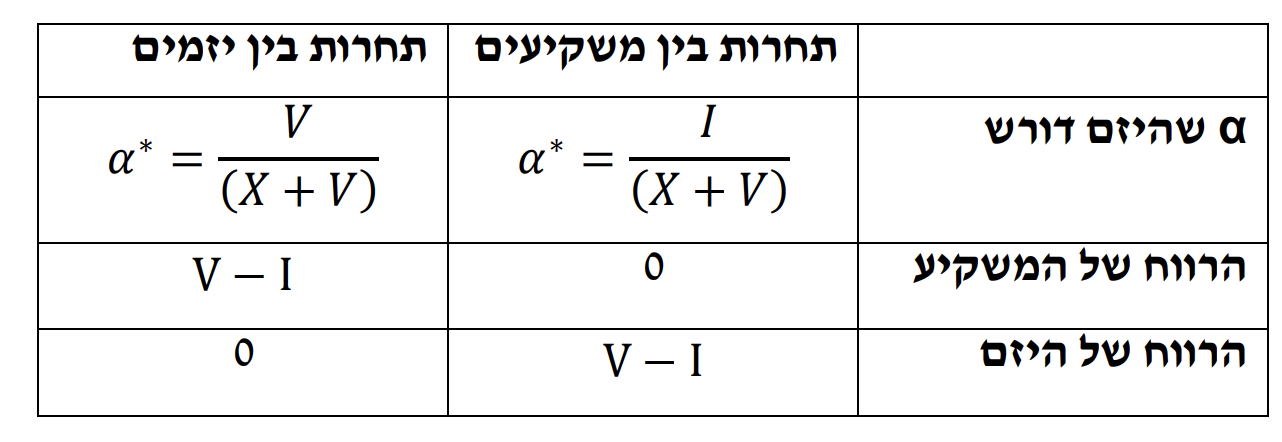
\includegraphics[width=\textwidth]{images/Screenshot 2023-12-03 at 19.35.55.png}
    \end{figure}

    \framebreak
    \begin{alertblock}{הערה}
    כל הדיבורים האלה היו כאשר האינפורמציה סימטרית, אבל מה קורה כאשר האינפורמציה אינה סימטרית?
        
    \end{alertblock}
   היזם תמיד יודע את $X$ והמשקיע או משקיעים מעריכים את הערך הנכס לפי תוחלת
   $$\mathbb{E}(X ) = \overline{X} = P \cdot X_H + \left(1-P\right) X_L $$
   ולכן החלק שמשקיעים ידרשו יגדל
    $$\overline{\alpha^*} \geq \frac{I}{X+V}$$

    \begin{alertblock}{תזכורת}
        $X$ הינו הערך האמיתי של הנכס, ו $\overline X$ הינו הערך המשוער שהמשקיעים נותנים לנכס
    \end{alertblock}
    \framebreak
    היזם צריך שאחרי השקעה ערך הנכס שישאר אצלו יהיה גבוה יותר מהערך במצב שלא ישקיעו בו (כלומר המצב המקורי)
    \begin{block}{רווח}
        $$\pi = \underbrace{(1-\alpha^*)\left(X +V \ \right)}_{\text{הערך החדש של הנכס שנשאר אצל היזם}} - \underbrace{X}_{\text{הערך המקורי של הנכס}} > 0 $$
        $$ \implies V - \frac{I \left(X + V \ \right)}{\bar X + V} > 0$$

        נסמן את $\theta = \dfrac{X+V}{\overline{X} + V}$ , נקבל :

        $$ V - I \cdot \theta > 0$$ 
    \end{block}
    \framebreak
    \begin{exampleblock}{מסקנות}
    \begin{itemize}
        \item כאשר $\theta < 1$ הפרויקט ייצא לפועל  (גם אם הוא לא כדאי) 
        \item לעומת זאת כאשר $\theta > 1$  לא בטוח שהפרויקט לא ייצא לפועל (גם אם הוא כדאי)
        \item חברות דירוג משמשות שחקן חשוב מאוד לצמצם את פער האינפורמציה בקרב משקיעים, הגורם שמרוויח והכי מעוניין בהצגת מידע אובייקטיבי למשקיעים הוא היזם ולכן הוא גם זה שיהיה שיממן את בדיקות הערך של חברות הדירוג
    \end{itemize}

	
\end{exampleblock}
\end{frame}
\end{RTL}
\end{document}